\documentclass[10pt]{article}
\usepackage[numbers]{natbib}
\usepackage{hyperref}
\usepackage[british]{babel}
\usepackage[utf8]{inputenc}
\usepackage[OT1]{fontenc}
\usepackage{amsfonts, amsmath, amsthm, amssymb}
\usepackage{graphicx}
\usepackage{listings}
\usepackage{physics}
\usepackage{empheq}
\usepackage[framemethod=tikz]{mdframed}
\usepackage{bbold}
\usepackage{tikz}
\usetikzlibrary{quantikz2}
\usepackage{braket}
\usepackage{titlesec}
\usepackage{adjustbox}
\usepackage{relsize}
\usepackage{bm}
\usepackage[most]{tcolorbox}
\numberwithin{equation}{section}

\usepackage{cancel}
\usepackage{wrapfig}
\usepackage{float}
\usepackage[margin=1in]{geometry}
\usepackage{xcolor}
\graphicspath{{../fig-files/notes-figs/}}

\hypersetup{
    colorlinks=true,
    citecolor=blue,
    filecolor=blue,
    linkcolor=blue,
    urlcolor=black
}
\newcounter{countCode}
\lstnewenvironment{code} [1][caption=Ponme caption, label=default]{%
	\renewcommand*{\lstlistingname}{Listado} 
	\setcounter{lstlisting}{\value{countCode}} 
	\lstset{ %
	language=java,
	basicstyle=\ttfamily\footnotesize,       % the size of the fonts that are used for the code
	numbers=left,                   % where to put the line-numbers
	numberstyle=\sc,      % the size of the fonts that are used for the line-numbers
	stepnumber=1,                   % the step between two line-numbers. 
	numbersep=5pt,                 % how far the line-numbers are from the code
	numberstyle=\color{red!50!blue},
    	backgroundcolor=\color{lightgray!20},
	rulecolor=\color{blue},
	keywordstyle=\color{red}\bfseries,
	showspaces=false,               % show spaces adding particular underscores
	showstringspaces=false,         % underline spaces within strings
	showtabs=false,                 % show tabs within strings adding particular underscores
	frame=single,                   % adds a frame around the code
	framexleftmargin=0mm,
	numberblanklines=false,
	xleftmargin=5pt,
	breaklines=true,
	breakatwhitespace=true,
	breakautoindent=true,
	captionpos=t,
	texcl=true,
	tabsize=2,                      % sets default tabsize to 3 spaces
	extendedchars=true,
	inputencoding=utf8, 
	escapechar=\%,
	morekeywords={print, println, size, background, strokeWeight, fill, line, rect, ellipse, triangle, arc, save, PI, HALF_PI, QUARTER_PI, TAU, TWO_PI, width, height,},
	emph=[1]{print,println,}, emphstyle=[1]{\color{blue}}, % Mis palabras clave.
	emph=[2]{width,height,}, emphstyle=[2]{\bf\color{violet}}, % Mis palabras clave.
	emph=[3]{PI, HALF_PI, QUARTER_PI, TAU, TWO_PI}, emphstyle=[3]\color{orange!50!violet}, % Mis palabras clave.
	emph=[4]{line, rect, ellipse, triangle, arc,}, emphstyle=[4]\color{green!70!black}, % Mis palabras clave.
	%emph=[5]{size, background, strokeWeight, fill,}, emphstyle=[5]{\tt \color{red!30!blue}}, % Mis palabras clave.
	%emph={[2]sqrt,baset}, emphstyle={[2]\color{blue}}, % f(sqrt(2)), sqrt a nivel 2 se pondrá azul
	#1}}{\addtocounter{countCode}{1}}


%\newtheorem{definition}{Definition}[section]

%\newcounter{fancydefinition}[section]
%\renewcommand{\thefancydefinition}{\thesection.\arabic{fancydefinition}}

%\newenvironment{fancydefinition}[1][]%
%  {\refstepcounter{fancydefinition}%
%\begin{definition}[Definition \thefancydefinition\ #1]}%
%  {\end{definition}}

\newtheoremstyle{defi}
  {\topsep}%
  {\topsep}%
  {\normalfont}%
  {}%
  {\bfseries}% 
  {:}%
  {.5em}%
  {\thmname{#1}\thmnote{~(#3)}}%
\theoremstyle{defi}
\newmdtheoremenv{definitioni}{Definition}[section]
\newmdtheoremenv[
hidealllines=true,
leftline=true,
innertopmargin=0pt,
innerbottommargin=0pt,
linewidth=4pt,
linecolor=gray!40,
innerrightmargin=0pt,
]{definitionii}{Definition}[section]



\newmdtheoremenv[
roundcorner=5pt,
innertopmargin=0pt,
innerbottommargin=5pt,
linewidth=4pt,
linecolor=gray!40,
]{definitioniii}{Definition}[section]

%%%%%%%%%%%%%%%%%%%%%%%%%%%%%%%%%%%%%%%%%%%%%%%%%%%%%%%%%%%%%%%%%%%%%%%%%%%%%%%%%%%%%%%%%%%%%%%%%%%%%%%%%%%%
% command for questions 
\newtcolorbox{question}{
freelance,
breakable,
before=\par\vspace{2\bigskipamount}\noindent,
after=\par\bigskip,
frame code={
  \node[
  anchor=south west,
  inner xsep=8pt,
  xshift=8pt,
  rounded corners=5pt,
  font=\bfseries\color{white},
  fill=gray] at (frame.north west) (tit) {\strut Question:};
  \draw[
  line width=3pt,
  rounded corners=5pt,gray
  ] (tit.west) -| (frame.south west) -- ([xshift=15pt]frame.south west);
},
interior code={},
top=2pt
}
%%%%%%%%%%%%%%%%%%%%%%%%%%%%%%%%%%%%%%%%%%%%%%%%%%%%%%%%%%%%%%%%%%%%%%%%%%%%%%%%%%%%%%%%%%%%%%%%%%%%%%%%%%%%



\bibliographystyle{apsrev4-1}
%\bibliographystyle{~/Desktop/revtex4-2.bst}
%\bibliographystyle{~/Documents/tex-packages/aps.bst}

\title{\textsf{\textbf{Lecture Notes on Quantum Computing and Quantum Information Theory}}}
\author{J. Gabriel Balarezo}
\date{\today}
\begin{document}
\maketitle \tableofcontents 

\begin{abstract}
  In this work we present a set of lecture notes on quantum computing and quantum information theory. The notes are based on the book by Nielsen and Chuang \cite{nielsen2010quantum}. The notes are intended to be used as a guide for a course on quantum computing and quantum information theory. Starting from the fundamentals of quantum computing (quantum mechanics review, definition of a qubit, algorithms and entangelment), this course covers a wide number of interesnting topics in quantum computing and quantum information.

\end{abstract}

\section{Fundamentals of Quantum Computing and Quantum Information}

\emph{Quantum Computing and Quantum Information} is undoubtedly a fascinating area, and is probably the path to follow in order to revolutionise the computational sciences. But before that, we must understand the classical representation of information.

Classically, we represent the information using discrete values, i.e bits. A bit is the smallest unit of information, and can have either a value of $0$ or $1$.  We may say that the classic representation of the information is "deterministic", since we can tell the state (it must be 0 or 1). Similarly, in quantum computing we also have the unit of information. We call it a \emph{qubit}, and unlike the classical bits, a qubit not only can take the discrete values of $0$ and $1$, but a linear combination\footnote{This purely quantum mechanical phenomena is called "superposition".} of them both
\begin{equation}
  \label{eq:1}
  \big|\psi\big>  = \alpha \big|0\big> + \beta \big|1\big>,
\end{equation}

More technically, we can say that a qubit $\big|\psi\big>$ is a superposition of two eigenstates\footnote{Two states {i, j} are said to be eigenstates if $\big<i\big|j\big>=0$.} $\big|0\big>$ and $\big|1\big>$ where $\alpha,\,\, \beta \in \mathbb{C}$ and $\big|\alpha\big|^2 + \big|\beta\big|^2 = 1$. We call this a probabilistic representation of the information.

\subsection{The Bloch Sphere}

The Bloch Sphere is a geometrical representation of the qubit. It is a unit sphere in $\mathbb{R}^3$ where the north and south poles represent the states $\big|0\big>$ and $\big|1\big>$ respectively. The equator of the sphere represents the superposition of the states $\big|0\big>$ and $\big|1\big>$. The states $\big|\psi\big>$ are represented by the points on the surface of the sphere. The Bloch Sphere is a useful tool to visualize the qubit states and their transformations.

\begin{equation}
  \label{eq:2}
  \big|\psi\big> = \cos\left(\frac{\varphi}{2}\right)\big|0\big> + e^{i\theta}\sin\left(\frac{\varphi}{2}\right)\big|1\big>,
\end{equation}
\begin{figure}[H]
  \centering
  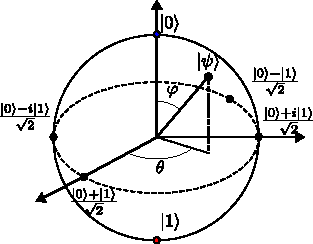
\includegraphics[width=0.5\textwidth]{fig-1-bloch-sphere.pdf}
  \caption{Bloch Sphere representation of a qubit state $\big|\psi\big>$.}
  \label{fig:bloch-sphere}
\end{figure}
where $\theta$ and $\varphi$ are the polar and azimuthal angles of the qubit state $\big|\psi\big>$.

\subsection{Classical Logic Gates}
\begin{figure}[H]
  \centering
  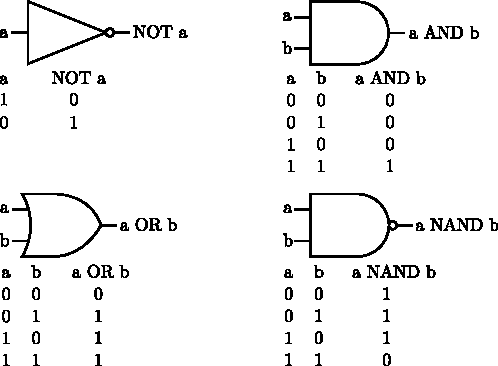
\includegraphics[width=0.5\textwidth]{logic-gates.pdf}
  \caption{Main logic gates.}
  \label{fig:logic-gates}
\end{figure}

In classical computing, we have the concept of logic gates. These are the basic building blocks of the digital circuits. The most common logic gates are the AND, OR, NOT, NAND, NOR, and XOR gates. In quantum computing, we also have the concept of quantum gates. These are the basic building blocks of the quantum circuits. The most common quantum gates are the Pauli gates, the Hadamard gate, the phase gate, the CNOT gate, and the Toffoli gate.

We say that the NAND gate is universal for classical computing, since any classical circuit can be built using only NAND gates. Similarly, the CNOT gate is universal for quantum computing, since any quantum circuit can be built using only CNOT gates. Even more specific, the NAND Gate is everyting necessary for a "Turin complete" model of computation.

\begin{definitionii}[Turin Complete]
  A model of computation is said to be Turin complete if it can be used to simulate any Turing machine. A Turing machine is a mathematical model of computation that defines an abstract machine that manipulates symbols on a strip of tape according to a table of rules. A Turing machine can simulate any computer algorithm, no matter how complicated.
\end{definitionii}

\subsection{Modelling Quantum Systems}
In order to depict the power of quantum computing, we must first provide an example where the classical computing fails. Let's consider the Many-body problem for atoms.

Consider a system of $N_I$ ions and $N_e$ electrons with ionic charges $eZ_I$, and where the ions are @ $\vec{R}_I$ and the electrons are @ $\vec{r}_i$. The electrons are the particles that we want to simulate. The electrons are fermions, and they obey the Pauli Exclusion Principle. This principle states that no two electrons can occupy the same quantum state. This means that the state of the system is a superposition of all the possible states of the electrons. This is a very hard problem to solve classically, since the number of states grows exponentially with the number of electrons. This is a problem that can be solved using quantum computing.

\begin{definitionii}[Born-Oppenheimer approximation]
The Born-Oppenheimer approximation is a foundational concept in molecular quantum mechanics. It allows for the separation of electronic and nuclear motions in molecules based on the vast difference in mass between electrons and nuclei. This approximation simplifies the Schrödinger equation by treating the electronic structure independently of nuclear motion. It enables the electronic wave function and energy to be solved first, considering the nuclei as fixed. Then, the nuclear motion can be treated semiclassically using the electronic energy as an effective potential. This approximation is crucial for understanding molecular structure and dynamics in computational chemistry and spectroscopy.
\end{definitionii}

We consider the wavefunction to be separable, i.e $\mathlarger{\Psi}(R_1, \dots, R_N; r_1, \dots, r_N)= \mathlarger{\chi}(R_1, \dots, R_N)\mathlarger{\psi}(r_1, \dots, r_N)$.  Where $\mathlarger{\chi}(R_1, \dots, R_N)$ is the nuclear wavefunction and $\mathlarger{\psi}(r_1, \dots, r_N)$ is the electronic wavefunction. Then, the Many-body Hamiltonian has the form

\begin{align}
  \label{eq:3}
  \hat{H} &= \frac{-\hbar^2}{2m_e}\sum_{i=1}^{N_e} \nabla_{\vec{r}_i}^2 + \frac{e^2}{4\pi\epsilon_0}\sum_{i=1}^{N_e}\sum_{j=i+1}^{N_e}\frac{1}{|\vec{r}_i - \vec{r}_j|} - 
  \frac{e^2}{4\pi\epsilon_0}\sum_{I=1}^{N_I}Z_I\sum_{i=1}^{N_e}\frac{1}{|\vec{r}_i - \vec{R}_I|} + \nonumber\\ 
  &- \frac{-\hbar^2}{2M_I}\sum_{I=1}^{N_I} \nabla_{\vec{R}_I}^2 + \frac{e^2}{4\pi\epsilon_0}\sum_{I=1}^{N_I}\sum_{J=I+1}^{N_I}\frac{Z_IZ_J}{|\vec{R}_I - \vec{R}_J|} 
\end{align}

If $\mathlarger{\Psi}(\vec{R}_1,\dots, \vec{R}_{N_I}; \vec{r}_1,\dots, \vec{r}_{N_e})$ is the full many-body wavefunction, then the Schrödinger equation for the system is 

\begin{equation}
  \label{eq:4}
  \hat{H}\mathlarger{\Psi} = \mathlarger{\chi}(R_1, \dots, R_N) \hat{H}_e\mathlarger{\psi}^{\vec{R}_1, \dots, \vec{R}_{N_I}}(r_1, \dots, r_{N_e})
  + \mathlarger{\psi}^{\vec{R}_1, \dots, \vec{R}_{N_I}}(r_1, \dots, r_{N_e})\hat{H}_n\mathlarger{\chi}(R_1, \dots, R_{N_I})
  \end{equation}
 where $\chi$ and $\psi$  are the ionic and electronic components of $\mathlarger{\Psi}$. 

\begin{mdframed}[backgroundcolor = gray!30,
  frametitle = Idea, roundcorner = 10pt]
  The electrons will relax to their ground state before the ionic core can be disturbed, so that wecan treat the system as classical ions with quantum mechanical electrons.
\end{mdframed}

\begin{equation*}
  \nabla^2 = \frac{\partial^2 f}{\partial x^2} + \frac{\partial^2 f}{\partial y^2} + \frac{\partial^2 f}{\partial z^2} \rightarrow \text{choose}\quad 
  \frac{\partial^2 f}{\partial x^2}  = \frac{\partial}{\partial x}\left(\frac{\partial f}{\partial x}\right)
\end{equation*}
writing the numerical approximation
\begin{equation}
  \label{eq:5}
  \frac{\partial^2 f}{\partial x^2} \approx \frac{f(x+h) - 2f(x) + f(x-h)}{h^2}
\end{equation}
and its matrix representation
\begin{equation}
  \label{eq:6}
  \nabla^2 f \approx \frac{1}{h^2}\begin{pmatrix}
    -2 & 1 & 0 & \dots & 0\\
    1 & -2 & 1 & \dots & 0\\
    0 & 1 & -2 & \dots & 0\\
    \vdots & \vdots & \vdots & \ddots & \vdots\\
    0 & 0 & 0 & \dots & -2
  \end{pmatrix} 
  \begin{pmatrix}
    f(x_0)\\
    f(x_1)\\
    f(x_2)\\
    \vdots\\
    f(x_n)
  \end{pmatrix}
\end{equation}
The electron-electron interaction is a two-point function. Now, let's compute the total energy of the system

\begin{align*}
  E_{\text{total}} &= E\big<\Psi\big|\Psi\big> = \big<\Psi\big|\hat{H}\big|\Psi\big>\\
&= \big<\chi\big|\chi\big>\big<\psi\big|\hat{H}_e\big|\psi\big> + \big<\psi\big|\psi\big>\big<\chi\big|\hat{H}_I\big|\chi\big>\\
  &= \big<\psi\big|\hat{T}_e\big|\psi\big> + \big<\psi\big|\hat{V}_{ee}\big|\psi\big> + \big<\psi\big|\hat{V}_{eI}\big|\psi\big> + \big<\chi\big|\hat{T}_I\big|\chi\big> + \big<\chi\big|\hat{V}_{II}\big|\chi\big> 
\end{align*}
therefore 

\begin{align}
  \label{eq:7}
  E(\vec{R}_1, \dots, \vec{R}_{N_I}) &= \big<\psi\big|\hat{T}_e\big|\psi\big> + \big<\psi\big|\hat{V}_{ee}\big|\psi\big> + \big<\psi\big|\hat{V}_{eI}\big|\psi\big>\nonumber\\
  &+ T_I(\vec{R}_1, \dots, \vec{R}_{N_I}) + V_{II}(\vec{R}_1, \dots, \vec{R}_{N_I})
\end{align}

Now, write the electron-electron contribution to the total energy 

\begin{align}
  \label{eq:8}
  \big<\psi(\vec{r}_1, \dots, \vec{r}_{N_e})\big|\sum_{i=1}^{N_e}\sum_{j=i+1}^{N_e}\frac{1}{|\vec{r}_i - \vec{r}_j|}\big|\psi(\vec{r}_1, \dots, \vec{r}_{N_e})\big> &= \iiint d^3 \vec{r}_{1}\dots\iiint d^3\vec{r}_{N_e}
  \sum_{i=1}^{N_e}\sum_{j=i+1}^{N_e}\frac{\big|\psi(\vec{r}_1, \dots, \vec{r}_{N_e})\big|^2}{|\vec{r}_i - \vec{r}_j|}\nonumber\\
  &= \sum_{i=1}^{N_e}\sum_{j=i+1}^{N_e}\int d^3\vec{r}_{1}\int d^3\vec{r}_{N_e}\frac{\big|\psi(\vec{r}_1, \dots, \vec{r}_{N_e})\big|^2}{|\vec{r}_i - \vec{r}_j|}\nonumber\\
  &= \sum_{i=1}^{N_e}\sum_{j=i+1}^{N_e}\int d^3\vec{r}_{1} \frac{\rho(\vec{r}_i, \vec{r}_{j})}{\big|\vec{r}_i - \vec{r}_j\big|}\nonumber\\
  &= \sum_{i=1}^{N_e}\sum_{j=i+1}^{N_e}\iint \frac{\rho(\vec{r'}) d^3\vec{r'}}{\big|\vec{r} - \vec{r'}\big|} \rho(\vec{r}) d^3\vec{r} + \int \frac{\delta E_{\text{ex}} \rho(\vec{r}) d^3\vec{r}}{\delta \rho}
\end{align}

The last term in Eq.\eqref{eq:8} is the exchange-correlation energy. The exchange energy is the energy associated with the Pauli exclusion principle. The correlation energy is the energy associated with the electron-electron interaction. 
Computing this term classically is very hard, since the number of states grows exponentially with the number of electrons. 
But, since quantum computing and quantum information is based on long-range correlations, we can compute this term using quantum computing.

\begin{question}
  How many bits of information are needed to describe an oxigen atom's many-body electronic wavefunction $\mathlarger{\psi}(r_1, \dots, r_{N_e})$?
\end{question}
\begin{itemize}
  \item Use a grid representation with a spacing of $h = 0.2$ \AA.
  \item Make each side of the box $L = 10$ \AA $= 1$ nm $= 50$ grid points. 
\end{itemize}

  \begin{equation*}
    \parbox{0.17\textwidth}{number of points} = \left(\frac{L}{h}\right)^3 = 50^3 \quad \text{points}
  \end{equation*}
\begin{equation*}
  \parbox{0.3\textwidth}{number of functional evaluations} = \left(\parbox{0.2\textwidth}{number of grid points}\right)^{N_e} = \left(\frac{L}{h}  \right)^{3\times N_e}
\end{equation*}
grows exponentially with the number of electrons. 

\begin{equation*}
 \# \text{data points} = 50^{24} \approx 5 \times 10^{24} = 5\times N_A
\end{equation*}

We can see that we will need the equivalent to $5$ Avogadro's numbers of bits to describe the many-body electronic wavefunction of an Oxigen atom.

\subsection{Quantum Logic Gates}
As aforementioned, for a system of computation to be "Turing complete" it needed only to implement the NAND gate. 
\begin{question}
  Can a quantum system of computation implement a NAND  gate?
\end{question}
Quantum systems obey time reversal symmetry (CAVEAT: this is not true for all quantum systems). This means that the time evolution of a quantum system is reversible. In order to construct the quantum logic gates we use quantum operators\footnote{Any quantum operator $\hat{\theta}$ is time reversible since it has an inverse.}.

So, we need to use "ancillary bits", i.e extra bits with a set initial value to "store" the result
% draw in latex a toffoli gate with states a and b and ancillary bit c = 0

\begin{figure}[H]
  \centering
  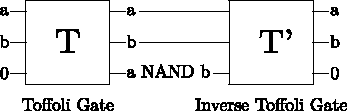
\includegraphics[width=0.4\textwidth]{toffoli-gate.pdf}
  \caption{Toffoli gate with ancillary bit 0.}
  \label{fig:toffoli-gate}
\end{figure}

The Toffoli gate provides a time reversible, i.e a invertable model for computation which is also "Turing complete". 

\begin{definitionii}[Efficiency]
  Time it takes to perform an algorithm $t(n)$ where n is the size of the input (space) is equal to a polynomial function
  \begin{equation*}
    t(n) = P(n) = \mathcal{O}(n^p), \quad p \in \mathbb{N}
  \end{equation*}
  or equivalently
\begin{equation*}
  \exists\, \text{M} \in \mathbb{R} \quad \text{such that} \quad t(n) \leq \text{M}n^p
\end{equation*}
  i.e $t(n)$ is bounded by $n^p$.
\end{definitionii}
\begin{definitionii}[Inefficient]
An algorithm is said to be inefficient if the time it takes grows exponentially as the size of the input, i.e,
\begin{equation*}
  t(n) = 2^n = \mathcal{O}(2^n)
\end{equation*}
\end{definitionii}

\subsection{Requirements for Quantum Computing}
So far, we have learned some definitions and a set of rules for a quantum system of computation to be "Turing complete". Now, we can state the requirements for a quantum system of computation.

\begin{enumerate}
\item Ability to prepare qubits in a well-defined initial input state, i.e  prepare either $\big|0\big>$ or $\big|1\big>$.
\item Ability to read the result of our algorithm, i.e measure the state of the qubit.
  \item Ability to prepare pure quantum superpositions, $\big|\psi\big> = \cos\left(\frac{\varphi}{2}\right)\big|0\big> + e^{i\theta}\sin\left(\frac{\varphi}{2}\right)\big|1\big>$.
  \item Toffoli\footnote{The 3-qubit Toffoli gate may be implemented using a combination of 2-qubit CNOT-gates.} gate implementation -two or three qubit gate.
\end{enumerate}

\begin{figure}[H]
  \centering
  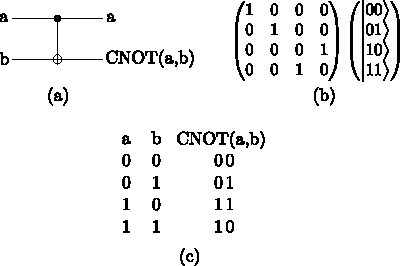
\includegraphics[width=0.5\textwidth]{cnot-gate.pdf}
  \caption{(a) represents the CNOT gate applied to the qubits a and b. (b) shows the matrix representation of the CNOT gate, and (c) shows its truth table.}
  \label{fig:quantum-computer}
\end{figure}

A single qubit (Eq. \eqref{eq:2}) can be represented as a position on the surface of the unit sphere (see Fig.\ref{fig:bloch-sphere}). Any combination of two qubits takes the form

\begin{equation}
  \label{eq:9}
  \big|\psi\big> = \alpha_{00} \big|00\big> + \alpha_{01} \big|01\big> + \alpha_{10} \big|10\big> + \alpha_{11} \big|11\big>
  \end{equation}

  where $\displaystyle{\sum_{i,j \in\{0, 1\}^2 }|\alpha_{ij}|^2 = 1}$. 

\subsection{Quantum Logic Gates}
\begin{mdframed}[backgroundcolor = gray!30,
  frametitle = Goal, roundcorner = 10pt]
  Can we make from the basis states $\big|0\big>$ or $\big|1\big>$ to the superposition of states, i.e onto the circle in the xy axis (frame) of the Bloch sphere?
  \end{mdframed}

  The answer is yes, we can. We can use the Hadamard gate to make the transformation.
\subsubsection{The Hadamard Gate}
The Hadamard gate creates superposition by putting the qubit $\big|0\big>$ and $\big|1\big>$  into a state where there is an equal probability of measuring 0 or 1. It's an essential gate in many quantum algorithms, including quantum teleportation and Grover's search algorithm.
  \begin{figure}[H]
    \centering
    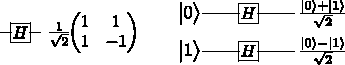
\includegraphics[width=0.45\textwidth]{hadamard-gate.pdf}
    \caption{Hadamard gate.}
    \label{fig:hadamard-gate}
  \end{figure}
If we apply the Hadamard gate to the qubit $\alpha |0\rangle + \beta |1\rangle$, we get

\begin{equation}
  \label{eq:10}
  \frac{1}{\sqrt{2}} \begin{pmatrix}
    1 & 1\\
    1 & -1
  \end{pmatrix}
  \begin{pmatrix}
    \alpha\\
    \beta
  \end{pmatrix}
  = \frac{\alpha + \beta}{\sqrt{2}}|0\rangle + \frac{\alpha - \beta}{\sqrt{2}}|1\rangle
\end{equation}
Similarly, we can apply the Hadamard gate to the pure superposition of states $\displaystyle{\frac{|0\rangle + i|1\rangle}{\sqrt{2}}}$,

\begin{align}
  \label{eq:11}
  \frac{1}{\sqrt{2}}\frac{1}{\sqrt{2}} \begin{pmatrix}
    1 & 1\\
    1 & -1
  \end{pmatrix}
  \begin{pmatrix}
    1\\
    i
  \end{pmatrix}
  =  \frac{1}{2}\begin{pmatrix}
    1 + i\\
    1 - i
  \end{pmatrix}
\end{align}
consider $(1 + i)$ and $(1 - i)$ as the complex numbers $z_1$ and $z_2$ respectively. Then, we can write the complex numbers as
$z_1 = \sqrt{2}e^{i\frac{\pi}{4}}$ and $z_2 = \sqrt{2}e^{-i\frac{\pi}{4}}$. So we can write the result in Eq.\eqref{eq:11} as 

\tikzset{operator/.append style={fill=red!20}}  

\begin{equation}
  \label{eq:12}
  \frac{|0\rangle + i|1\rangle}{\sqrt{2}}
  \begin{quantikz}[column sep=0.5cm, thin lines]
  & \gate{H} & 
  \end{quantikz}  
   = \frac{\sqrt{2}\exp(i\pi/4)|0\rangle +\sqrt{2} \exp(-i\pi/4)|1\rangle}{2}
\end{equation}
we can also multiply this state by a phase factor, i.e $\exp(i\pi/4)$, which is a global phase factor. This means it does not change the state of the qubit

\begin{equation*}
  \frac{\sqrt{2}\exp(i\pi/4)|0\rangle +\sqrt{2} \exp(-i\pi/4)|1\rangle}{2}  \exp(i\pi/4) = \frac{|0\rangle - i|1\rangle}{\sqrt{2}} 
\end{equation*} 

\begin{equation}
  \label{eq:13}
  \frac{|0\rangle + i|1\rangle}{\sqrt{2}} 
  \begin{quantikz}[column sep=0.5cm, thin lines]
  & \gate{H} &
  \end{quantikz}
   = \frac{|0\rangle - i|1\rangle}{\sqrt{2}}
\end{equation}

\subsubsection{The $\pi/8$ Gate} 
The $\frac{\pi}{8}$ gate introduces a phase shift of $\frac{\pi}{4}$ (or $\frac{\pi}{8}$ radians) to the state $|1\rangle$, leaving $|0\rangle$ unchanged. Mathematically, it applies the transformation:

\begin{equation}
  \label{eq:14}
  \begin{quantikz}[column sep=0.5cm, thin lines]
    & \gate{T} &
  \end{quantikz}
  = \begin{pmatrix}
    1 & 0\\
    0 & e^{i\pi/4}
   \end{pmatrix}
\end{equation}

\subsubsection{Phase Gate}
The phase gate introduces a phase shift of $\frac{\pi}{2}$ (or $\frac{\pi}{2}$ radians) to the state $|1\rangle$, leaving $|0\rangle$ unchanged. Mathematically, it applies the transformation:

\begin{equation}
  \label{eq:15}
  \begin{quantikz}[column sep=0.5cm, thin lines]
    & \gate{S} &
  \end{quantikz}
  = \begin{pmatrix}
    1 & 0\\ 
    0 & i\\ 
    \end{pmatrix}
    \equiv 
    \begin{quantikz}[column sep=0.5cm, thin lines]
      & \gate{T} & \gate{T} &
    \end{quantikz}
\end{equation}
\subsubsection{Pauli-Z Gate}

\begin{equation}
  \label{eq:16}
  \begin{quantikz}[column sep=0.5cm, thin lines]
    & \gate{Z} &
  \end{quantikz}
  = \begin{pmatrix}
    1 & 0\\ 
    0 & -1\\ 
    \end{pmatrix}
\end{equation}
The Pauli-Z gate generates a half-turn in the Bloch sphere about the $z$ axis. With respect to the computational basis, the $Z$ gate flips the phase of the $|1\rangle$ state relative to the $|0\rangle$ state.

\subsubsection{Pauli-X Gate}
\begin{equation}
  \label{eq:17}
  \begin{quantikz}[column sep=0.5cm, thin lines]
    & \gate{X} &
  \end{quantikz}
  = \begin{pmatrix}
    0 & 1\\ 
    1 & 0\\ 
    \end{pmatrix}
\end{equation}
The X-gate is also known as a bit-flip gate. It generates a half-turn in the Bloch sphere about the $x$ axis.

With respect to the computational basis, the $X$ gate is equivalent to a classical NOT operation, or logical negation. The computation basis states are interchanged, so that $|0\rangle$ becomes $|1\rangle$ and $|1\rangle$ becomes $|0\rangle$. 

\subsubsection{Pauli-Y Gate}

\begin{equation}
  \label{eq:18}
  \begin{quantikz}[column sep=0.5cm, thin lines]
    & \gate{Y} &
  \end{quantikz}
  = \begin{pmatrix}
    0 & -i\\ 
    i & 0\\ 
    \end{pmatrix}
\end{equation}

The Pauli-Y gate generates a half-turn in the Bloch sphere about the $y$ axis. This gate can be thought as a combination of $X$ and $Z$ gates, $Y = -iZX$. With respect to the computational basis, we interchange the zero and one states and apply a relative phase flip.


The Hadamard Gate, $\pi/8$ Gate and CNOT gate are called universal gates since they are sufficient to implement quantum computation. 

\subsection{Bell's States}
The Bell states, named after physicist John S. Bell, are a set of four maximally entangled quantum states of two qubits. They represent fundamental examples of quantum entanglement, wherein the states of two particles become interdependent regardless of the distance between them. 

These states, denoted as $\beta_{00}$, $\beta_{01}$, $\beta_{10}$, and $\beta_{11}$, demonstrate distinct patterns of correlation between the qubits, characterized by specific superpositions of the basis states. For instance, the $\beta_{00}$ state represents an equal superposition of both qubits being in the state $|0\rangle$ or $|1\rangle$, while the $\beta_{01}$ state has opposite signs in the superposition. 

The importance of Bell states lies in their pivotal role in various quantum information processing tasks, including quantum teleportation, superdense coding, and quantum cryptography. They serve as essential resources for enabling secure communication, efficient information transmission, and the implementation of quantum algorithms. The general diagram for Bell's states  is here 

% write the bell 00 state using quantikz 
\begin{equation}
  \label{eq:19}
  \begin{quantikz} 
    \ket{i} \gategroup[wires=2, steps=1, style={dashed, rounded corners,fill = blue!20, inner sep=3pt},background, label style={label position=below, yshift=-0.5cm}]{pure states}& \gate{H} & \ctrl{1} &\rstick[2]{$\ket{B_{ij}}$, $i,j$ $\in$ \{0,1  \} } \\
     \ket{j} &          & \targ{}  & 
  \end{quantikz}
\end{equation}
even more generallly, we can write the Bell states as

\begin{equation}
  \label{eq:20}
  \ket{B_{ij}}  =  
  \begin{quantikz} 
    \lstick[2]{$\ket{B_{00}}$} &  & & \\ 
    & \gate{X^{i}}  & \gate{Z^j} &
  \end{quantikz}
\end{equation}
\newpage
\begin{mdframed}[backgroundcolor = gray!30,
  frametitle = Bell's states, roundcorner = 10pt]
\begin{equation}
  \label{eq:21}
  %draw the bell 00 state using quantikz 
  \begin{quantikz} 
    \lstick{$\ket{0}$} & \gate{H} & \ctrl{1} & \rstick[2]{$\frac{1}{\sqrt{2}}(\ket{00} + \ket{11})$} \\
    \lstick{$\ket{0}$} & \qw & \targ{} &
  \end{quantikz}
  = \ket{B_{00}}
\end{equation}
\begin{equation}
  \label{eq:22}
  %draw the bell 01 state using quantikz2 
  \begin{quantikz} 
    \lstick{$\ket{0}$} & \gate{H} & \ctrl{1} & \rstick[2]{$\frac{1}{\sqrt{2}}(\ket{00} - \ket{11})$} \\
    \lstick{$\ket{1}$} & \qw & \targ{} &
  \end{quantikz}
  = \ket{B_{01}}
\end{equation}
\begin{equation}
  \label{eq:23}
  %draw the bell 10 state using quantikz3
  \begin{quantikz} 
    \lstick{$\ket{1}$} & \gate{H} & \ctrl{1} & \rstick[2]{$\frac{1}{\sqrt{2}}(\ket{10} + \ket{01})$} \\
    \lstick{$\ket{0}$} & \qw & \targ{} &
  \end{quantikz}
  = \ket{B_{10}}
\end{equation}
\begin{equation}
  \label{eq:24}
  %draw the bell 11 state using quantikz4
  \begin{quantikz} 
    \lstick{$\ket{1}$} & \gate{H} & \ctrl{1} & \rstick[2]{$\frac{1}{\sqrt{2}}(\ket{10} - \ket{01})$} \\
    \lstick{$\ket{1}$} & \qw & \targ{} &
  \end{quantikz}
  = \ket{B_{11}}
\end{equation}
  \end{mdframed}

\subsection{Quantum Teleportation}

Quantum teleportation is a process by which the state of a qubit can be transmitted from one location to another, with the help of two classical bits and an entangled pair of qubits. The process involves three parties: the sender, the receiver, and the qubit to be teleported. 
For the matter of this example, let's consider the state of the qubit to be teleported as $\ket{\psi} = \alpha\ket{0} + \beta\ket{1}$. The sender and receiver share an entangled pair of qubits in the Bell state $\ket{B_{00}} = \frac{1}{\sqrt{2}}(\ket{00} + \ket{11})$. The sender performs a Bell measurement on the qubit to be teleported and their half of the entangled pair. The result of the Bell measurement is two classical bits, which are sent to the receiver. The receiver then applies a series of quantum gates based on the classical bits received, to transform their half of the entangled pair into the original state of the qubit to be teleported.

% draw the quantum teleportation circuit using quantikz2 
\begin{equation}
  \label{eq:25}
\begin{quantikz}
  \lstick[2]{Alice} \ket{\psi} && \ctrl{1} & \gate{H} & \meter{M_1} & \setwiretype{c} & \cwbend{2} \\
 \lstick[2]{$\ket{B_{00}}$}    && \targ{}  &         & \meter{M_2}  & \cwbend{1} \setwiretype{c}  \\
\lstick{Bob}           &&          &         &              & \gate{X^{M_2}}   & \gate{Z^{M_1}} 
\end{quantikz}
\end{equation}

Now, let's do the math behind the quantum teleportation. We start with the state of the qubit to be teleported $\ket{\psi} = \alpha\ket{0} + \beta\ket{1}$ and the entangled pair in the Bell state $\ket{B_{00}} = \frac{1}{\sqrt{2}}(\ket{00} + \ket{11})$. The total state of the system is given by

\begin{equation}
  \label{eq:26}
  \ket{\psi} \otimes \ket{B_{00}} = \frac{1}{\sqrt{2}}(\alpha\ket{0} + \beta\ket{1})\otimes(\ket{00} + \ket{11})
\end{equation}

Expanding the tensor product, we get 

\begin{equation}
  \label{eq:27}
  \frac{1}{\sqrt{2}}(\alpha\ket{0}\otimes\ket{00} + \alpha\ket{0}\otimes\ket{11} + \beta\ket{1}\otimes\ket{00} + \beta\ket{1}\otimes\ket{11})
\end{equation}

Now, we apply the Hadamard gate to the first qubit of the qubit to be teleported and the CNOT gate to the two qubits. The state of the system after these operations is

\begin{equation}
  \label{eq:28}
  \frac{1}{2}(\alpha\ket{0}\otimes(\ket{0} + \ket{1}) + \alpha\ket{1}\otimes(\ket{0} - \ket{1}) + \beta\ket{0}\otimes(\ket{0} + \ket{1}) + \beta\ket{1}\otimes(\ket{0} - \ket{1}))
\end{equation}

Now, we measure the two qubits and send the results to the receiver. The receiver then applies the Pauli-X and Pauli-Z gates to their qubit based on the classical bits received. The state of the receiver's qubit after these operations is

\begin{equation}
  \label{eq:29}
  \frac{1}{2}(\alpha\ket{0} + \beta\ket{1})
\end{equation}

This is the original state of the qubit to be teleported, $\ket{\psi} = \alpha\ket{0} + \beta\ket{1}$. Thus, the quantum teleportation process has successfully transmitted the state of the qubit from the sender to the receiver.




\newpage 
\bibliography{references-2}
%\bibliography{~/Library/texmf/bibtex/bib/zotero}

\end{document}

